The standard way to access the vast magnitude of data available on UniProtKB it by using the websites text search.
The website provides a search bar in the UniProt banner in which a query can be filled in.
The query syntax accepts terms of specific fields and combines them using boolean logic.
A manual is provided on the website,
but a more convenient method is to use the query builder.
It lets the user build a query step by step by providing drop down lists for the available fields
(Fig. \ref{fig:query_builder}).
Once the 'search' button is clicked, the query is shown in the search bar in the appropriate syntax and results are given in a table like format
(Fig. \ref{fig:query_results}).
The pencil symbol lets the user choose which columns are shown.
Once satisfied, results can be downloaded in one of multiple formats, the most important being:
a fasta file of all the selected protein sequences,
an Excel or tab separated text file containing the fields of choice (e.g. id, length, and sequence) for every selected protein,
or a XML file.
The latter is not meant to be read by humans in its raw format, but can be easily parsed.
It contains all information available on UniProtKB for the selected proteins.


~\begin{figure}[h!]
	~\begin{subfigure}[b]{\linewidth}
		\centering
		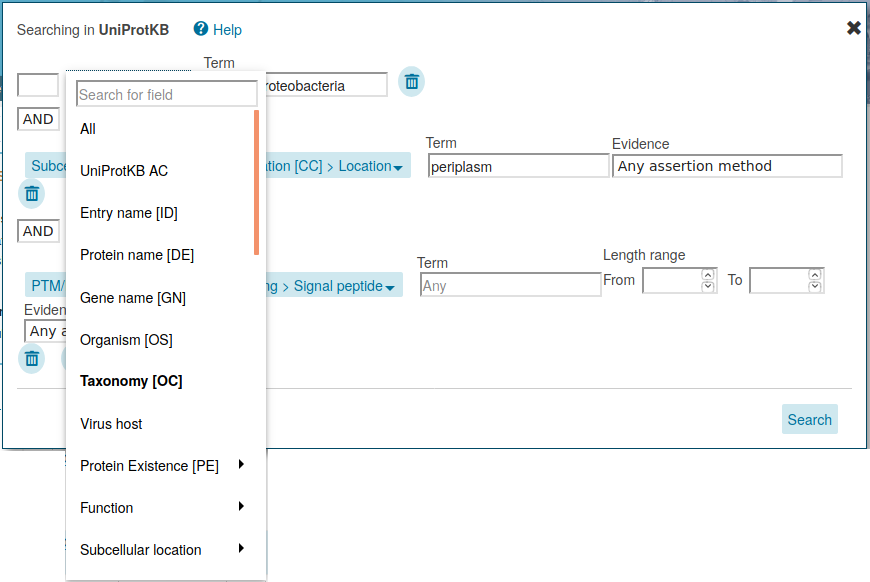
\includegraphics[width=\linewidth,height=0.3\textheight,keepaspectratio]
			{./literature_review/UniProtKB/text_search/img/query_builder.png}
		\caption{Query Builder}
		\label{fig:query_builder}
	~\end{subfigure}
	~\begin{subfigure}[b]{\linewidth}
		\centering
		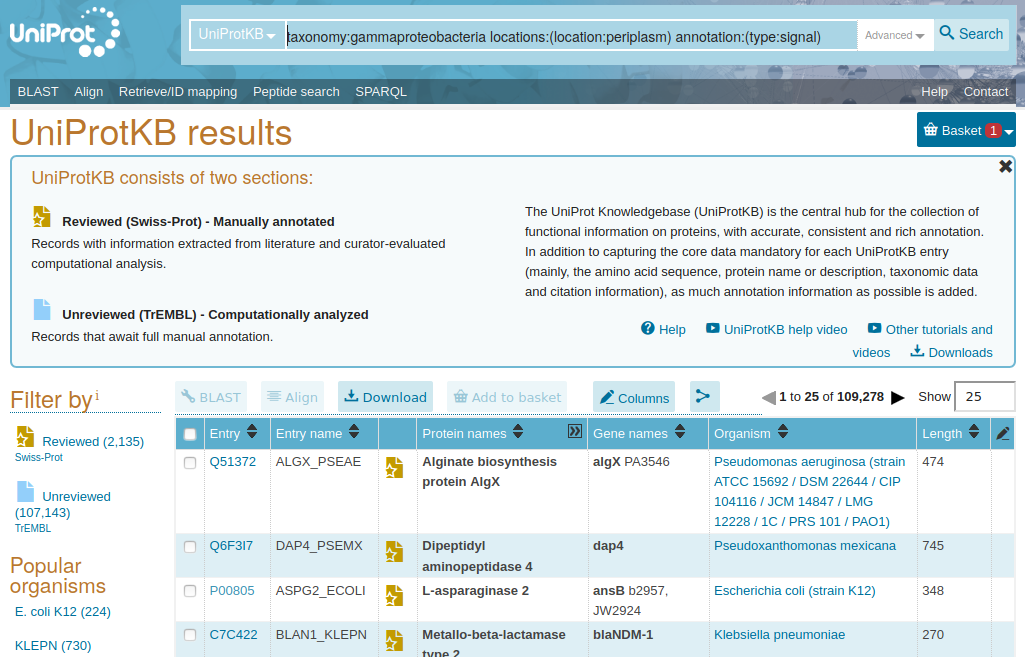
\includegraphics[width=\linewidth, height=0.5\textheight,keepaspectratio]
			{./literature_review/UniProtKB/text_search/img/query_results.png}
		\caption{Query Results}
		\label{fig:query_results}
	~\end{subfigure}
	\caption{
		\textbf{The UniProtKB website text search.}
		The vast UniProtKB database can be accessed by text search.
		\textbf{a.} The search bar accepts a boolean style of query syntax, 
		which can by build step by step with the Query Builder.
		\textbf{b.} Results are shown in a table like format.
		(Screenshot from https://www.uniprot.org/).
		}
~\end{figure}
